\documentclass[a4,12pt]{scrartcl}

%Basic 
\usepackage[utf8]{inputenc}
\usepackage[ngerman]{babel}
\usepackage[T1]{fontenc}
\usepackage{float}
\usepackage[bottom = 3.50cm]{geometry}

%Titel Seite
\title{CLOUD INFRASTRUCTURE}
\subtitle{Lab-08}
\author{Giorgio Vincenti \and Samuel Krieg}
\date{\today}


%Kopf, Fusszeile
\usepackage{fancyhdr}
\pagestyle{fancy}
\lhead{ \begin{picture}(0,0) \put(0,0){
\includegraphics[width=3cm]{./pictures/hsrlogo.png}} \end{picture}}
\chead{}
\rhead{Seite \thepage}
\lfoot{Cloud Infrastructure \\Lab-08}
\cfoot{Giorgio Vincenti \and Samuel Krieg}
\rfoot{\today}
\renewcommand{\headrulewidth}{0.4pt}

%Bilder
\usepackage{graphicx}

%Tabellen
\usepackage{booktabs}

%Codesnippets
\usepackage{listings}
\lstset{language=python} 

%Hyperlinks
\usepackage{hyperref}

%Querformat für eine Seite
\usepackage{lscape}
\usepackage{rotating}
\usepackage{pdflscape}

%Temp
\usepackage{lipsum}



\begin{document}

\clearpage\maketitle
\thispagestyle{empty}
\tableofcontents
\newpage

\section{Mininet}
Wurde aus der Aufgabenstellung entnommen: \\
\\
Mininet is a network emulator which creates a network of virtual hosts, switches, controllers, and links. Mininet hosts run standard Linux network software, and its switches support OpenFlow for highly flexible custom routing and Software-Defined Networking.\\
\\
Mininet supports research, development, learning, prototyping, testing, debugging, and any other tasks that could benefit from having a complete experimental network on a laptop or other PC.\\
\\
\textbf{Mininet:}
\begin{itemize}
\item Provides a simple and inexpensive network testbed for developing OpenFlow applications
\item Enables multiple concurrent developers to work independently on the same topology
\item Supports system-level regression tests, which are repeatable and easily packaged
\item Enables complex topology testing, without the need to wire up a physical network
\item Includes a CLI that is topology-aware and OpenFlow-aware, for debugging or running network-wide tests
\item Supports arbitrary custom topologies, and includes a basic set of parametrized topologies
\item is usable out of the box without programming, but
\item also Provides a straightforward and extensible Python API for network creation and experimentation
\end{itemize}

\noindent Mininet provides an easy way to get correct system behavior (and, to the extent supported by your hardware, performance) and to experiment with topologies.
Mininet networks run real code including standard Unix/Linux network applications as well as the real Linux kernel and network stack (including any kernel extensions which you may have available, as long as they are compatible with network namespaces.)

\subsection{Aufgaben}
Create a custom topology script for clos fabric
\begin{itemize}
\item Tow parameter for Leaf and Spine
\item Layer2 or Layer3
\end{itemize}

\section{Mininet Script (Python)}
\begin{lstlisting}
#!/usr/bin/python

from mininet.topo import Topo
from cmd import Cmd

class LeafAndSpine(Topo):
    def __init__(self, spine=2, leaf=2):
        Topo.__init__(self)

        spines = {}
        for s in range(spine):
            spines[s] = self.addSwitch('spine%s'%(s+1))
            Cmd('sh ovs-vsctl set-fail-mode spine%s standalone'%(s+1))
            Cmd('sh ovs-vsctl set Bridge spine%s stp_enable=true'%(s+1))

        for l in range(leaf):
            leafSwitch = self.addSwitch('leaf%s'%(l+1))
            Cmd('sh ovs-vsctl set-fail-mode leaf%s standalone'%(l+1))
            Cmd('sh ovs-vsctl set Bridge leaf%s stp_enable=true'%(l+1))
            
            host = self.addHost('h%s' % (l+1),ip="10.10.1.%s"%(l+1))
            self.addLink(host,leafSwitch)

            for s in range(spine):
                self.addLink(leafSwitch, spines[s])

topos = {'LeafAndSpine':(lambda spine,leaf:LeafAndSpine(spine, leaf))}
\end{lstlisting}

\subsection{Infrastruktur}
Das Script und die Umgebung wurde in einer virtuellen Maschine, mit Linux Ubuntu Server, getestet. Die einzige Voraussetzung für das testen ist, dass Mininet installiert ist. Wir gehen nicht auf die Einzelheiten ein.

\subsection{Layer}
Mininet Infrastruktur wurde im Layer2 betrieben,. Um Loops zu vermeiden, wurde auf Spanning-Tree auf den Switches aktiviert. 

\subsection{Mininet starten, mit Parameter}
Um Mininet mit folgenden Script aufzustarten, ist die Angabe des Scripts bei Start von Mininet notwendig. 
\begin{lstlisting}
#Startet Mininet mit Script - wobei x = Anzahl Spines, y = Anzahl Leafs
#LeafAndSpineSwitchTopo_v2.py = Scriptname 
sudo mn --custom LeafAndSpineSwitchTopo_v2.py --topo=LeafAndSpine,x,y 
\end{lstlisting}

\subsubsection{Mininet-Topo mit 2x Spines und 4x Leafs}
In diesem Beispiel wird Mininet mithilfe des Scripts aufgesetzt, mit dem man die Anzahl Spines und Leafs als Parameter mitgeben kann. Pro Leaf wird automatisch einen Host hinzugefügt. 
\begin{figure} [H]
	\begin{center}
	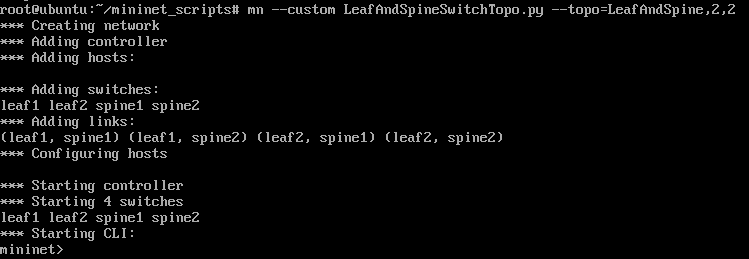
\includegraphics[width=1.00\textwidth]{./pictures/example.png}
	\caption{Screenshot: Mininet Config mit Script}
	\label{x}
	\end{center}
\end{figure} 

\subsubsection{Test: pingall}
Hier einige Ping-Tests die mithilfe von pingall durchgefüht wurden. 
\begin{figure} [H]
	\begin{center}
	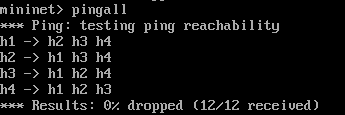
\includegraphics[width=0.60\textwidth]{./pictures/example_ping.png}
	\caption{Screenshot: pingall}
	\label{x}
	\end{center}
\end{figure} 
\end{document}